\section{Methodology}
\subsection{Attack Pipeline}
We study clean-label poisoning attacks against feature-based malware classifiers.
Let $\boldsymbol{x} \in \mathcal{X}$ denote a feature vector extracted from a benign or malware sample, and let $y \in \{0, 1\}$ denote its label, where 0 and 1 indicate benign and malware, respectively.
A trigger is represented as a set of feature-value assignments $T = \{(f_{1}, v_{1}), (f_{2}, v_{2}), \cdots, (f_{k}, v_{k})\}$, where $f_{i}$ is a selected trigger feature, and $v_{i}$ is the value assigned to that feature.
For an input sample $\boldsymbol{x}$, trigger injection overwrites the original values of the selected features with the corresponding trigger values, producing a triggered sample $\boldsymbol{x}_{T}$.

\begin{figure}[t]
    \centering
    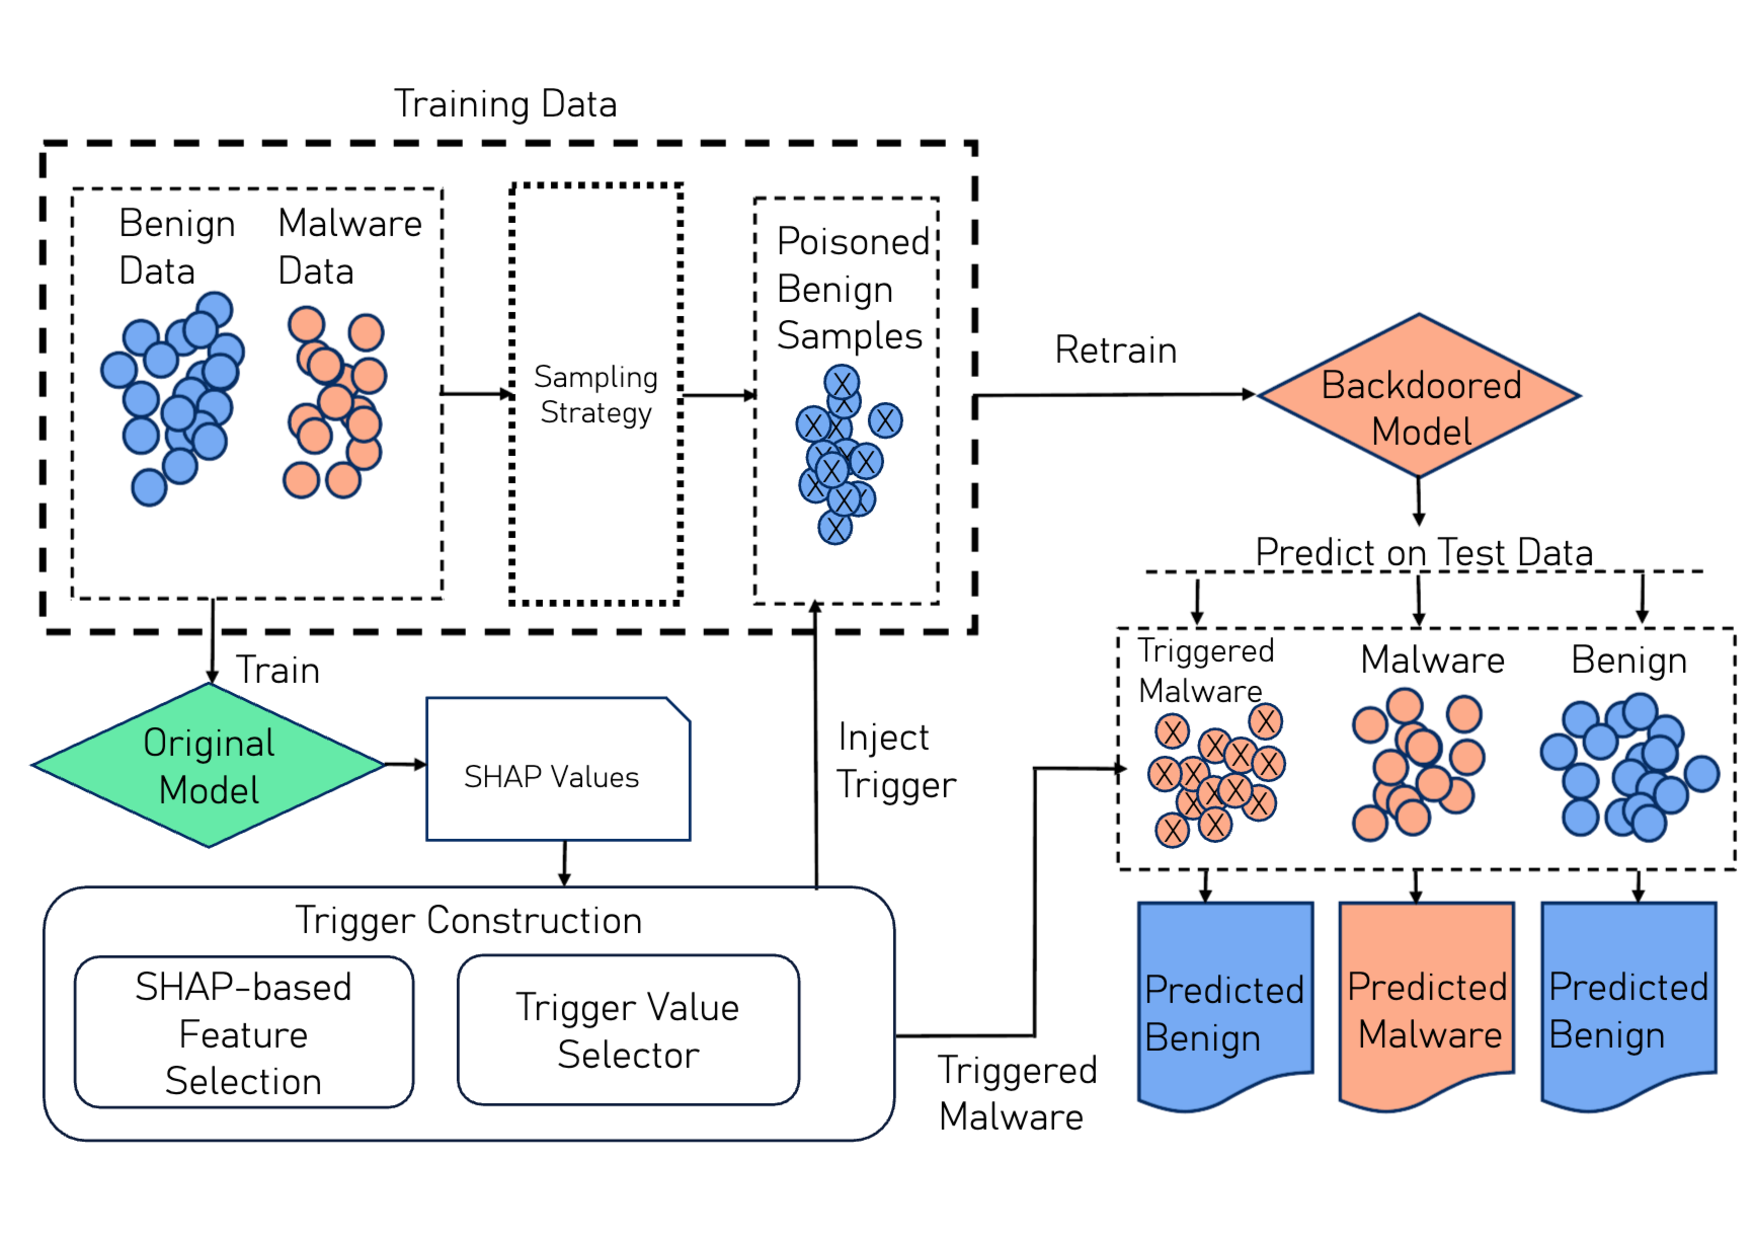
\includegraphics[width=\hsize]{figure/attack_pipeline.pdf}
    \caption{Overview of the clean-label backdoor poisoning pipeline.}
    \label{fig:attack_pipeline}
\end{figure}

Fig.~\ref{fig:attack_pipeline} shows the overall attack pipeline used in this work.
Our pipeline follows the explanation-guided clean-label backdoor attack setting~\cite{severi}.
We first train a clean baseline classifier on the original training data and then compute feature importance scores using SHAP values.
A fixed set of trigger features is selected based on the largest aggregated absolute SHAP values across training samples, subject to feature-space feasibility constraints so that only feasible features are used to construct the backdoor trigger.
For each experiment, we use one value-selection strategy to choose the trigger values from the original training data for the selected trigger features. 
The resulting trigger is injected into a subset of benign training samples without changing their labels.
The classifier is then retrained on the poisoned training set to obtain the backdoored model.
Finally, we evaluate the backdoored model on clean test samples and triggered malware samples.
The attack objective is to cause triggered malware samples to evade detection while preserving normal performance on clean samples; accordingly, we use attack success rate as the primary attack-effectiveness metric.

\subsection{Trigger Value Selection Strategies}
The main focus of this work is trigger value selection.
After the set of trigger features $F_{T} = \{f_{1}, f_{2}, \cdots, f_{k}\}$ is fixed, a value selector determines which value $v_{i}$ should be assigned to each selected feature $f_{i}$.
In addition to the Severi-derived selectors~\cite{severi}, we introduce five extended selectors: FrequencyBoundedSignedSHAP, LowSignedSHAP, CorrCountAbsSHAP, BenignPrototype, and QuantileDistribution.
These selectors are designed to test whether signed SHAP direction, frequency bounds, co-occurrence support, benign prototypes, or empirical quantiles can change the effectiveness--detectability relationship.
We group the value selectors according to the main signal used by each selector: frequency or distribution, SHAP contribution, and co-occurrence or prototype support.
These categories are not mutually exclusive; some selectors combine multiple signals, such as frequency and SHAP magnitude, or signed SHAP contribution and co-occurrence.
Table~\ref{tab:value_selectors} summarizes the value-selection strategies evaluated in this work.

\subsubsection{Frequency- and Quantile-based Selectors}
The selectors choose values according to how common, rare, or distributionally positioned they are in benign data.
Rare-value selection places the trigger in a sparse region of the feature space, following the intuition of the MinPopulation method~\cite{severi}.
Such values may give the trigger stronger leverage over the decision boundary, but they may also create more distinctive patterns that are easier to detect.
Frequency-bounded and quantile-based selectors are included to test whether controlling the rarity or empirical position of trigger values changes the effectiveness--detectability profiles.
For QuantileDistribution, we evaluated Q05, Q50, and Q95, and report Q95 in the main tables because it gave the strongest and most consistent results.

\subsubsection{SHAP-based Selectors}
The selectors use feature attribution scores to estimate how candidate values contribute to the classifier's decision.
Following the intuition of the CountAbsSHAP method~\cite{severi}, magnitude-based selectors use feature importance scores to identify values with low absolute class-specific contributions.
For malware-class explanations, negative SHAP values push the classifier's decision toward the benign class.
Signed SHAP selectors use this direction of contribution and select values that are expected to push predictions toward the benign class.
We evaluate whether using signed SHAP values produces stronger or less detectable triggers than magnitude-only criteria.

\subsubsection{Co-occurrence- and Prototype-based Selectors}
The selectors consider whether selected feature-value pairs naturally appear together in benign samples.
This follows the intuition of the CombinedSHAP method~\cite{severi}, which greedily selects feature-value pairs that remain consistent with existing benign samples.
Unlike independent value selection, co-occurrence-aware selection aims to preserve relationships among selected feature values so that the trigger better blends into the benign distribution.
Previous work has noted that independently selected values may not correspond to naturally occurring benign patterns, while Combined-style selection is designed to align with existing benign-oriented regions~\cite{severi,ho_sanitization}.

\begin{table*}[!t]
    \centering
    \caption{Summary of trigger value-selection strategies.}
    \label{tab:value_selectors}
    \begin{tabularx}{\textwidth}{>{\raggedright\arraybackslash}p{2.2cm}
    >{\raggedright\arraybackslash}p{3.2cm}
    >{\raggedright\arraybackslash}X
    >{\raggedright\arraybackslash}p{3.2cm}}
        \toprule
        \textbf{Source} & \textbf{Selector} & \textbf{Main principle} & \textbf{Category} \\
        \midrule
        Severi-derived & MinPopulation & Selects rare observed values. & Frequency / rarity \\
        Severi-derived & CountAbsSHAP & Balances value frequency and low absolute SHAP contribution. & Frequency + SHAP magnitude \\
        Severi-derived & CombinedSHAP & Greedily selects benign-oriented co-occurring feature-value pairs. & Signed SHAP + co-occurrence \\
        This work & FreqBoundedSigned & Selects benign-oriented values within a frequency range. & Frequency + signed SHAP \\
        This work & LowSignedSHAP & Selects values with a benign-oriented signed contribution. & Signed SHAP \\
        This work & CorrCountAbsSHAP & Considers low absolute SHAP values with co-occurrence support. & SHAP magnitude + co-occurrence \\
        This work & BenignPrototype & Selects values from representative benign patterns. & Prototype / co-occurrence \\
        This work & QuantileDistribution & Selects values from fixed empirical distribution positions. & Distribution baseline \\
        \bottomrule
    \end{tabularx}
\end{table*}
